% First draft: general quadrilateral ABCD with side midpoints E/F/M/N (schematic outer vertices, exact midpoints).
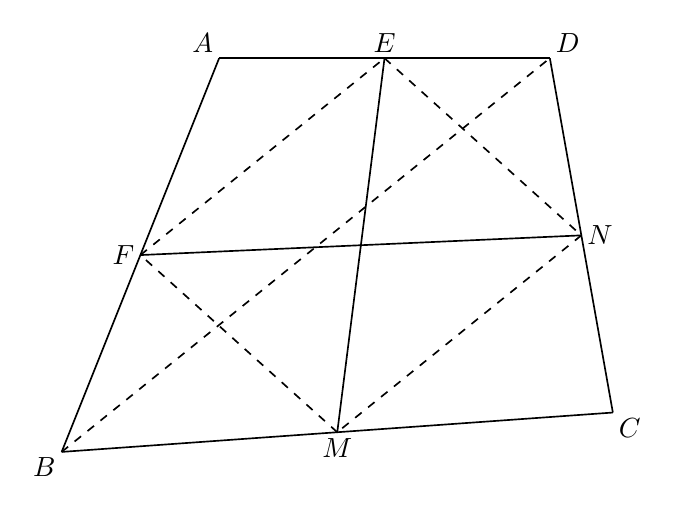
\begin{tikzpicture}[x=1cm,y=1cm,font=\normalsize,
 geometry edge/.style={solid,line width=.6pt},
 geometry mark/.style={solid,line width=.6pt},
 geometry label/.style={font=\normalsize,inner sep=2pt}]
\coordinate (A) at (0,4);
\coordinate (B) at (-2,-1);
\coordinate (C) at (5,-0.5);
\coordinate (D) at (4.2,4);
\coordinate (E) at (2.1,4);
\coordinate (F) at (-1,1.5);
\coordinate (M) at (1.5,-0.75);
\coordinate (N) at (4.6,1.75);
\draw[geometry edge] (A)--(B);
\draw[geometry edge] (B)--(C);
\draw[geometry edge] (C)--(D);
\draw[geometry edge] (D)--(A);
\draw[geometry edge] (E)--(M);
\draw[geometry edge] (F)--(N);
\draw[geometry edge,dashed] (F)--(E);
\draw[geometry edge,dashed] (E)--(N);
\draw[geometry edge,dashed] (N)--(M);
\draw[geometry edge,dashed] (M)--(F);
\draw[geometry edge,dashed] (B)--(D);
\node[geometry label,above left] at (A) {$A$};
\node[geometry label,below left] at (B) {$B$};
\node[geometry label,below right] at (C) {$C$};
\node[geometry label,above right] at (D) {$D$};
\node[geometry label,above] at (E) {$E$};
\node[geometry label,left] at (F) {$F$};
\node[geometry label,below] at (M) {$M$};
\node[geometry label,right] at (N) {$N$};
\end{tikzpicture}
